
\begin{figure}[h]
	\centering
	\begin{subfigure}[b]{0.3\textwidth}
		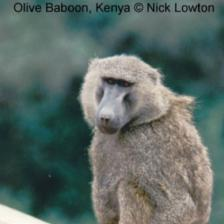
\includegraphics[width=.9\textwidth]{img/examples/appendix/n02486410_08484}
		\caption{Orginalne zdjęcie}  \label{}
	\end{subfigure}
	\begin{subfigure}[b]{0.3\textwidth}
		\centering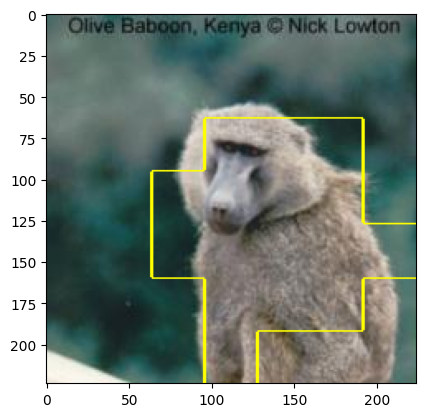
\includegraphics[width=.9\textwidth]{img/examples/appendix/n02486410_08484_gradcam}
		\caption{GradCAM}  \label{}
	\end{subfigure}
	\begin{subfigure}[b]{0.3\textwidth}
		\centering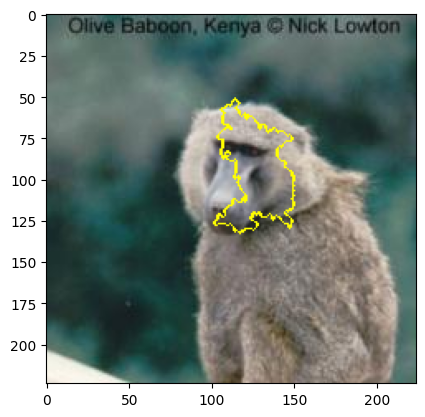
\includegraphics[width=.9\textwidth]{img/examples/appendix/n02486410_08484_lime}
		\caption{LIME}
	\end{subfigure}
	\caption{Przykład spójności wyjaśnień GradCAM i LIME bliskiej średniej - IoU=0.178527}
	\label{}
\end{figure}
\begin{figure}[h]
	\centering
	\begin{subfigure}[b]{0.3\textwidth}
		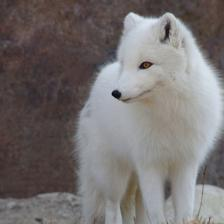
\includegraphics[width=.9\textwidth]{img/examples/appendix/n02120079_49517}
		\caption{Orginalne zdjęcie}  \label{}
	\end{subfigure}
	\begin{subfigure}[b]{0.3\textwidth}
		\centering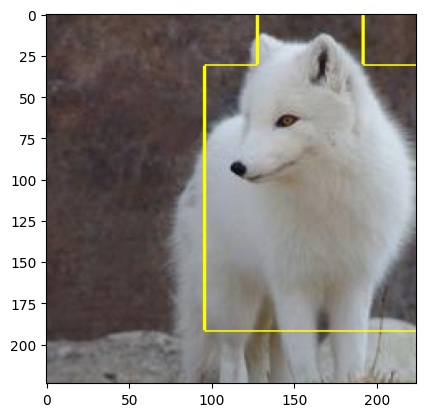
\includegraphics[width=.9\textwidth]{img/examples/appendix/n02120079_49517_gradcam}
		\caption{GradCAM}  \label{}
	\end{subfigure}
	\begin{subfigure}[b]{0.3\textwidth}
		\centering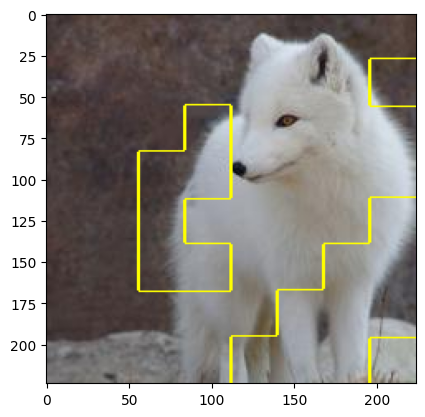
\includegraphics[width=.9\textwidth]{img/examples/appendix/n02120079_49517_shap}
		\caption{SHAP}
	\end{subfigure}
	\caption{Przykład spójności wyjaśnień GradCAM i SHAP bliskiej średniej - IoU=0.111111}
	\label{}
\end{figure}
\begin{figure}[h]
	\centering
	\begin{subfigure}[b]{0.3\textwidth}
		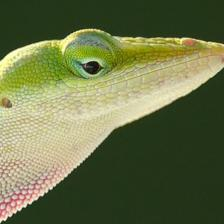
\includegraphics[width=.9\textwidth]{img/examples/appendix/n01682714_14308}
		\caption{Orginalne zdjęcie}  \label{}
	\end{subfigure}
	\begin{subfigure}[b]{0.3\textwidth}
		\centering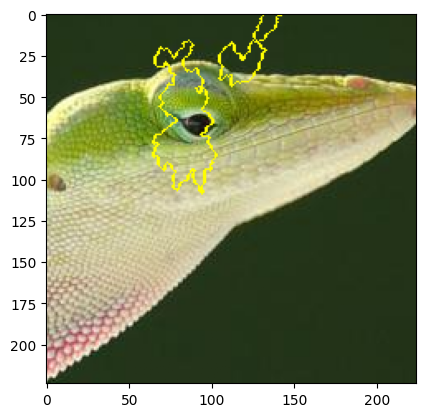
\includegraphics[width=.9\textwidth]{img/examples/appendix/n01682714_14308_lime}
		\caption{LIME}  \label{}
	\end{subfigure}
	\begin{subfigure}[b]{0.3\textwidth}
		\centering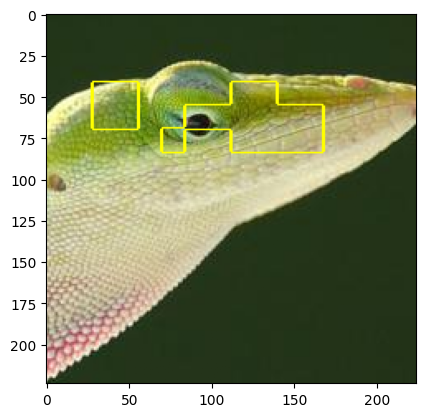
\includegraphics[width=.9\textwidth]{img/examples/appendix/n01682714_14308_shap}
		\caption{SHAP}
	\end{subfigure}
	\caption{Przykład spójności wyjaśnień LIME i SHAP bliskiej średniej - IoU=0.072499}
	\label{}
\end{figure}

\begin{figure}[h]
	\centering
	\begin{subfigure}[b]{0.3\textwidth}
		
\includegraphics[width=.9\textwidth]{img/examples/appendix/n03884397_34878}
		\caption{Orginalne zdjęcie}  \label{}
	\end{subfigure}
	\begin{subfigure}[b]{0.3\textwidth}
		\centering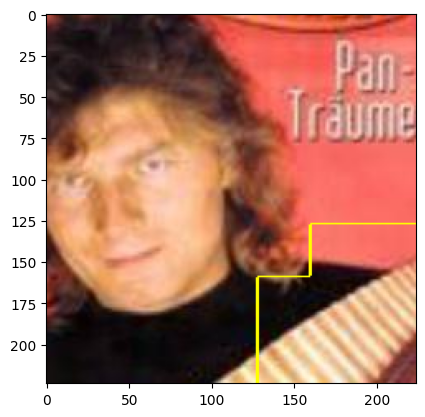
\includegraphics[width=.9\textwidth]{img/examples/appendix/n03884397_34878_gradcam}
		\caption{GradCAM}  \label{}
	\end{subfigure}
	\begin{subfigure}[b]{0.3\textwidth}
		\centering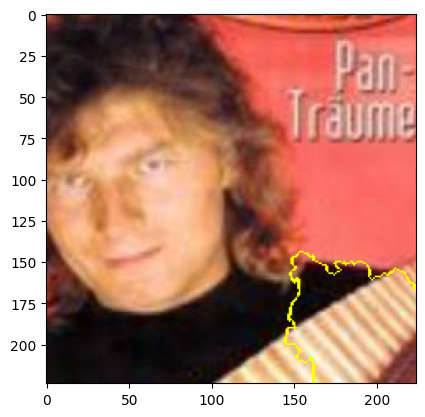
\includegraphics[width=.9\textwidth]{img/examples/appendix/n03884397_34878_lime}
		\caption{LIME}
	\end{subfigure}
	\caption{Przykład spójności wyjaśnień GradCAM i LIME odstające pozytywnie - IoU=0.688791}
	\label{}
\end{figure}
\begin{figure}[h]
	\centering
	\begin{subfigure}[b]{0.3\textwidth}
		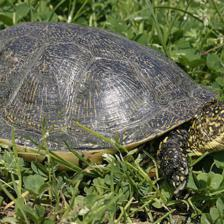
\includegraphics[width=.9\textwidth]{img/examples/appendix/n01667778_32805}
		\caption{Orginalne zdjęcie}  \label{}
	\end{subfigure}
	\begin{subfigure}[b]{0.3\textwidth}
		\centering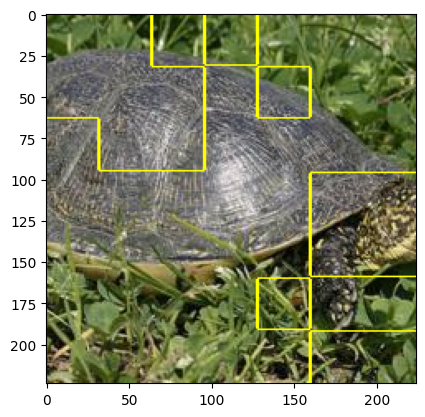
\includegraphics[width=.9\textwidth]{img/examples/appendix/n01667778_32805_gradcam}
		\caption{GradCAM}  \label{}
	\end{subfigure}
	\begin{subfigure}[b]{0.3\textwidth}
		\centering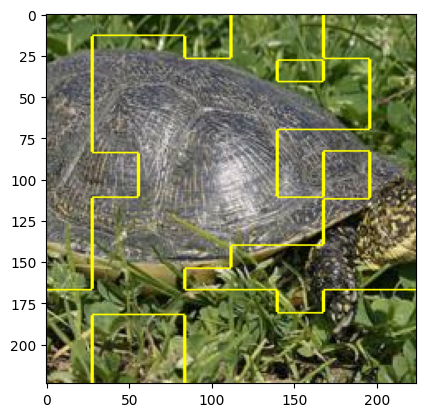
\includegraphics[width=.9\textwidth]{img/examples/appendix/n01667778_32805_shap}
		\caption{SHAP}
	\end{subfigure}
	\caption{Przykład spójności wyjaśnień GradCAM i SHAP odstające pozytywnie - IoU=0.46888}
	\label{}
\end{figure}
\begin{figure}[h]
	\centering
	\begin{subfigure}[b]{0.3\textwidth}
		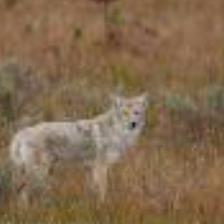
\includegraphics[width=.9\textwidth]{img/examples/appendix/n02114855_39555}
		\caption{Orginalne zdjęcie}  \label{}
	\end{subfigure}
	\begin{subfigure}[b]{0.3\textwidth}
		\centering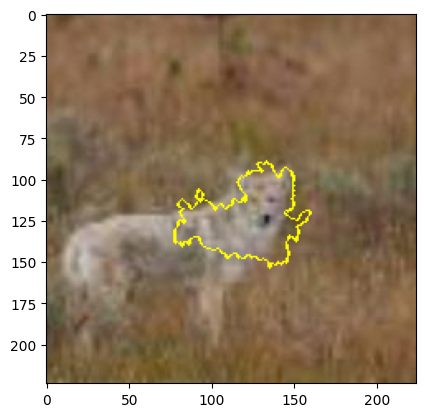
\includegraphics[width=.9\textwidth]{img/examples/appendix/n02114855_39555_lime}
		\caption{LIME}  \label{}
	\end{subfigure}
	\begin{subfigure}[b]{0.3\textwidth}
		\centering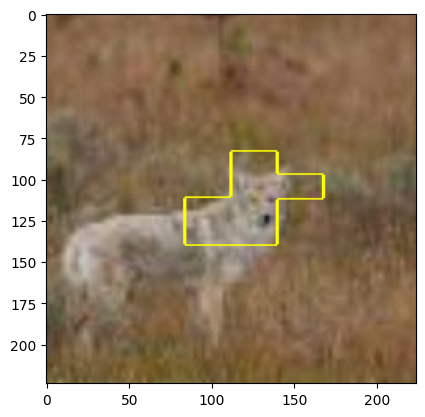
\includegraphics[width=.9\textwidth]{img/examples/appendix/n02114855_39555_shap}
		\caption{SHAP}
	\end{subfigure}
	\caption{Przykład spójności wyjaśnień LIME i SHAP odstające pozytywnie - IoU=0.53489}
	\label{}
\end{figure}

\begin{figure}[h]
	\centering
	\begin{subfigure}[b]{0.3\textwidth}
		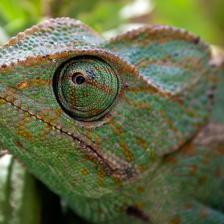
\includegraphics[width=.9\textwidth]{img/examples/appendix/n01694178_23707}
		\caption{Orginalne zdjęcie}  \label{}
	\end{subfigure}
	\begin{subfigure}[b]{0.3\textwidth}
		\centering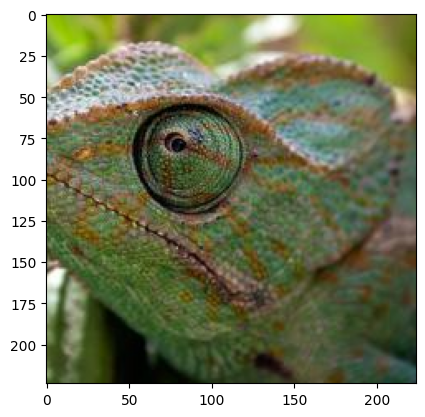
\includegraphics[width=.9\textwidth]{img/examples/appendix/n01694178_23707_gradcam}
		\caption{GradCAM}  \label{}
	\end{subfigure}
	\begin{subfigure}[b]{0.3\textwidth}
		\centering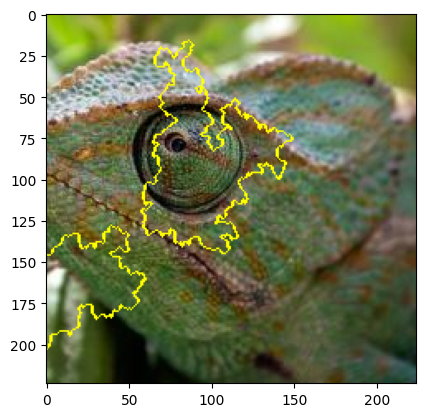
\includegraphics[width=.9\textwidth]{img/examples/appendix/n01694178_23707_lime}
		\caption{LIME}
	\end{subfigure}
	\caption{Przykład spójności wyjaśnień GradCAM i LIME odstające negatywnie - IoU=0.0}
	\label{}
\end{figure}
\begin{figure}[h]
	\centering
	\begin{subfigure}[b]{0.3\textwidth}
		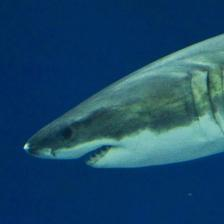
\includegraphics[width=.9\textwidth]{img/examples/appendix/n01484850_19435}
		\caption{Orginalne zdjęcie}  \label{}
	\end{subfigure}
	\begin{subfigure}[b]{0.3\textwidth}
		\centering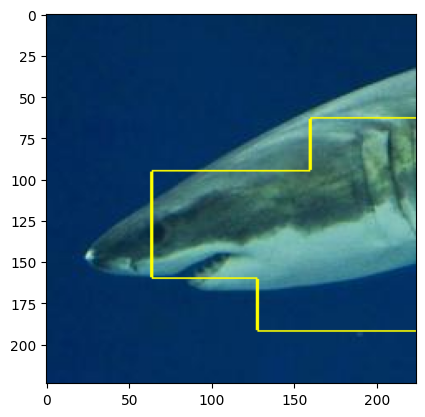
\includegraphics[width=.9\textwidth]{img/examples/appendix/n01484850_19435_gradcam}
		\caption{GradCAM}  \label{}
	\end{subfigure}
	\begin{subfigure}[b]{0.3\textwidth}
		\centering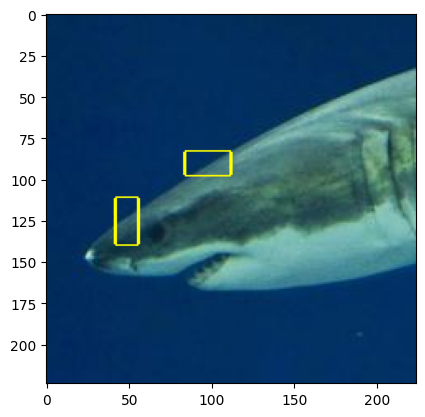
\includegraphics[width=.9\textwidth]{img/examples/appendix/n01484850_19435_shap}
		\caption{SHAP}
	\end{subfigure}
	\caption{Przykład spójności wyjaśnień GradCAM i SHAP  odstające negatywnie- IoU=0.0}
	\label{}
\end{figure}
\begin{figure}[h]
	\centering
	\begin{subfigure}[b]{0.3\textwidth}
		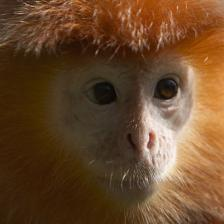
\includegraphics[width=.9\textwidth]{img/examples/appendix/n02488291_05090}
		\caption{Orginalne zdjęcie}  \label{}
	\end{subfigure}
	\begin{subfigure}[b]{0.3\textwidth}
		\centering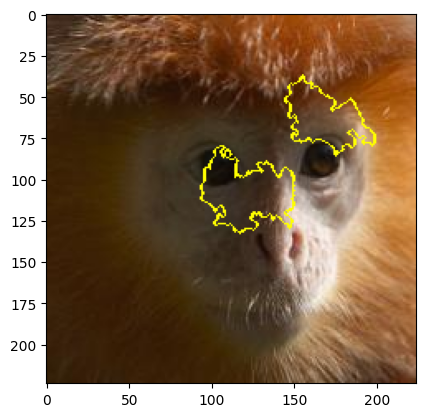
\includegraphics[width=.9\textwidth]{img/examples/appendix/n02488291_05090_lime}
		\caption{LIME}  \label{}
	\end{subfigure}
	\begin{subfigure}[b]{0.3\textwidth}
		\centering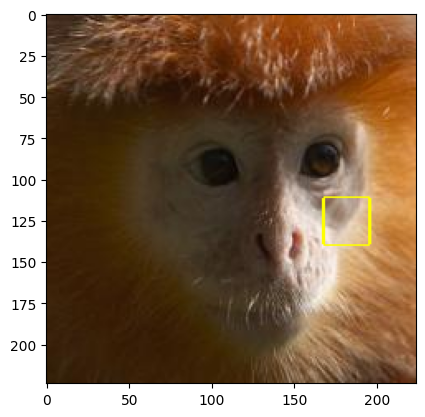
\includegraphics[width=.9\textwidth]{img/examples/appendix/n02488291_05090_shap}
		\caption{SHAP}
	\end{subfigure}
	\caption{Przykład spójności wyjaśnień LIME i SHAP odstające negatywnie - IoU=0.0}
	\label{}
\end{figure}

